%%%%%%%%%%%%%%%%%%%%%%%%%%%%%%%%%%%%%%%%%%%%%%%%%%%%%%%%%%%%%%%%%%%%%%%%
\section{The tail law}\label{sec:tail}
%%%%%%%%%%%%%%%%%%%%%%%%%%%%%%%%%%%%%%%%%%%%%%%%%%%%%%%%%%%%%%%%%%%%%%%%

\subsection{Statements}

The exact identity~\eqref{eq:identity} turns determinant weights into the tail of the size $N$ at a
shifted parameter. That tail is the following.

\begin{theorem}[tail law]\label{thm:tail}
For every $Q\ge2$ and every fixed $\varepsilon>0$,
\[
\lim_{n\to\infty}\frac{\log\Prob_Q(N\ge n)}{\log n}\;=\;-\frac4{\gamma^2},
\]
where $\gamma=Q-\sqrt{Q^2-4}$ as in~\eqref{eq:Q}; at the critical endpoint $Q=2$, $\gamma=2$ and
the limit is $-1$.
\end{theorem}

This is a logarithmic asymptotic, $\Prob(N\ge n)=n^{-4/\gamma^2+o(1)}$, not a limit of
$n^{4/\gamma^2}\Prob(N\ge n)$. At $Q=2$ we also prove $\E[N]<\infty$, so there the tail is not a
constant times $1/n$. With Proposition~\ref{prop:identity}, the theorem gives the KPZ formula in
the model.

\begin{theorem}[the KPZ curve]\label{thm:kpz}
Take the base parameter $Q_0^2=25/6$, that is $c=0$. For every real $k\ge-1/2$, put
$Q_k^2=Q_0^2+k/3$ and
\[
W_k(n)=\sum_{n'\ge n}\Bigl(\frac{Q_k}{Q_0}\Bigr)^{n'}A_0^{-k}\,n'^{-k/3}\;
\E_{Q_0}\bigl[(\ldet)^k;\,N=n'\bigr],
\]
the weight of surfaces with at least $n$ squares under the $k$-th power of the determinant, with
both compensations of Section~\ref{sec:tilt}. Then $W_k(n)=n^{-x_k+o(1)}$, where
\[
x_k+\frac1{x_k}=\frac{13+2k}{6},\qquad x_k\ge1,\qquad
x_k=\frac{13+2k+\sqrt{(13+2k)^2-144}}{12}.
\]
At $k=0,1,2$ this gives $x_k=3/2$, $2$ and $\xstar=(17+\sqrt{145})/12$, so $1+x_2=\astar$.
\end{theorem}

\begin{proof}
By~\eqref{eq:identity}, $W_k(n)=\Prob_{Q_k}(N\ge n)$; this needs $Q_k\ge2$, which is
$25/6+k/3\ge4$, that is $k\ge-1/2$. By Theorem~\ref{thm:tail} at parameter $Q_k$, the tail
exponent is $x_k=4/\gamma_k^2$ with $Q_k=2/\gamma_k+\gamma_k/2$, and by~\eqref{eq:xQ},
$x_k+1/x_k=Q_k^2-2=(13+2k)/6$.
\end{proof}

\begin{figure}[b]
\centering
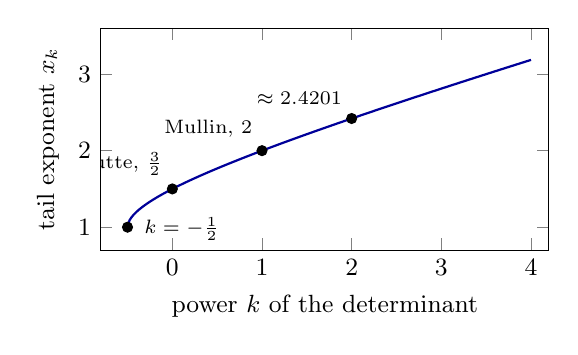
\begin{tikzpicture}
\begin{axis}[width=0.6\textwidth,height=4.4cm,xmin=-0.8,xmax=4.2,ymin=0.7,ymax=3.6,
  xlabel={power $k$ of the determinant},ylabel={tail exponent $x_k$},
  tick label style={font=\small},label style={font=\small},
  xtick={0,1,2,3,4},ytick={1,2,3}]
\addplot[domain=-0.5:4,samples=200,thick,blue!60!black]
  {(13+2*x+sqrt(max(0,(13+2*x)^2-144)))/12};
\addplot[only marks,mark=*,mark size=1.8pt] coordinates {(-0.5,1) (0,1.5) (1,2) (2,2.42013)};
\node[font=\scriptsize,anchor=west] at (axis cs:-0.42,0.98) {$k=-\frac12$};
\node[font=\scriptsize,anchor=south east] at (axis cs:0,1.55) {Tutte, $\frac32$};
\node[font=\scriptsize,anchor=south east] at (axis cs:1,2.05) {Mullin, $2$};
\node[font=\scriptsize,anchor=south east] at (axis cs:2,2.47) {$\xstar\approx2.4201$};
\end{axis}
\end{tikzpicture}
\caption{The KPZ curve of Theorem~\ref{thm:kpz}, with central charge $c=-2k$. Marked: the
critical endpoint, the bare surface, one spanning tree, and the analog of two spanning trees,
whose exponent is the meander value $\xstar=\astar-1$.}
\label{fig:kpz}
\end{figure}

Figure~\ref{fig:kpz} shows the curve. Three caveats. First, the result concerns cumulative weights,
up to factors $n^{o(1)}$; a local upper bound $\Prob(N=n)\le n^{-1-4/\gamma^2+o(1)}$ along
$n\equiv1\pmod3$ is also proved, and the local lower bound is open. So at $k=2$ it proves the
tail exponent $\xstar$, not the local exponent $\astar=1+\xstar$. Second, it is a statement for
each fixed $k$ and cannot be differentiated in $k$. Third, it concerns a continuum model in which
spanning trees are replaced by a determinant, not meanders or tree-weighted planar maps.

\subsection{A heuristic for the exponent}\label{sec:heuristic}

The proofs make the following heuristic rigorous. The size $N$ is large only if the field is
unusually high somewhere. The cheapest way is to make a single square very high and let its
descendants multiply. Two exponential rates describe this.

\emph{The cost of a high square.} Measure the growth of an average along nested squares per level,
in units of $\log2$, and call it the \emph{slope}. A square of depth $j$ whose average has slope
$\lambda$, that is $h_S\approx\lambda\,j\log2$, has height $H(S)\approx(\lambda-Q)\,j\log2$ by~\eqref{eq:height}.
There are $4^j$ squares at depth $j$, and a normal variable of variance $j\log2$ exceeds
$\lambda j\log2$ with probability about $2^{-j\lambda^2/2}$. So the expected number of squares
at height $y=(\lambda-Q)j\log2$ is about
\[
2^{\,j(2-\lambda^2/2)}=\exp\Bigl(-y\,\frac{\lambda^2/2-2}{\lambda-Q}\Bigr).
\]
Minimizing the ratio over $\lambda>Q$ gives the condition $\lambda^2/2-Q\lambda+2=0$, whose root
above $Q$ is $\lambda_+=Q+\sqrt{Q^2-4}$, and there the ratio equals $\lambda_+$. So a square of
height $y$ appears with probability about $e^{-\lambda_+y}$.

\emph{The yield of a high square.} Start from one square of height $y$ and follow its descendants
whose averages grow with slope $\theta$ below the threshold slope $Q$. Along such a path the
height decreases by $(Q-\theta)\log2$ per level, so the path stays active for about
$j'=y/((Q-\theta)\log2)$ levels. The expected number of such descendants is
\[
2^{\,j'(2-\theta^2/2)}=\exp\Bigl(y\,\frac{2-\theta^2/2}{Q-\theta}\Bigr).
\]
Maximizing over $\theta$ gives the same condition, $\theta^2/2-Q\theta+2=0$, now with the root
below $Q$, which is $\lambda_-=Q-\sqrt{Q^2-4}=\gamma$, and there the ratio equals $\gamma$. So a
square of height $y$ produces about $e^{\gamma y}$ final squares; this count is typical, not only an
expectation, because $\gamma<2$.

Putting $n=e^{\gamma y}$, the probability of at least $n$ squares is about
$e^{-\lambda_+y}=n^{-\lambda_+/\gamma}$. Since $\lambda_+\lambda_-=4$, the exponent is
$\lambda_+/\gamma=4/\gamma^2$. In words: the two roots of one quadratic,
\begin{equation}\label{eq:quadratic}
\psi(\theta)=2-Q\theta+\frac{\theta^2}2,\qquad \psi(\gamma)=\psi(4/\gamma)=0,
\end{equation}
are the rate at which height is gained cheaply and the rate at which it is spent productively,
and their ratio is the KPZ exponent. The function $\psi$ also governs the upper bound: the number
of active squares at depth $j$ is at most $2^{j\psi(\theta)}$ times a random factor with controlled
moments, for each $\theta$, as the next section shows.

The proof has four parts: the upper bound for $Q>2$, by moments of Gaussian multiplicative chaos
(Section~\ref{sec:upper}, nearly in full); the upper bound at $Q=2$, by a Brownian estimate
(Section~\ref{sec:upper}); and the lower bounds for $Q>2$ and $Q=2$, by a second-moment count of
high squares with many descendants (sketched in Section~\ref{sec:lower}).
